\section{Code completion with NLMs}
Language modelling faces a difficult problem when it comes to code completion. There are local (to only one block of code) and very long distance dependencies in coding, such as initializing a variable only once per function. One approach involved merging a model employing pointer networks with attention, which was shown to perform better at simulating long distance dependencies than RNNs and LSTMs~\cite{ccnlm}.

% \subsection{Pointer Networks (Ptr-Net)}
% Pointer networks~\cite{pointer} are built on top of modified attention mechanism with pointers to input words. Figure~\ref{fig:1b} illustrates these pointers.

% \begin{figure}[hbt!]
% \centering 
% \subfloat[Sequence-to-Sequence.\label{fig:1a}]{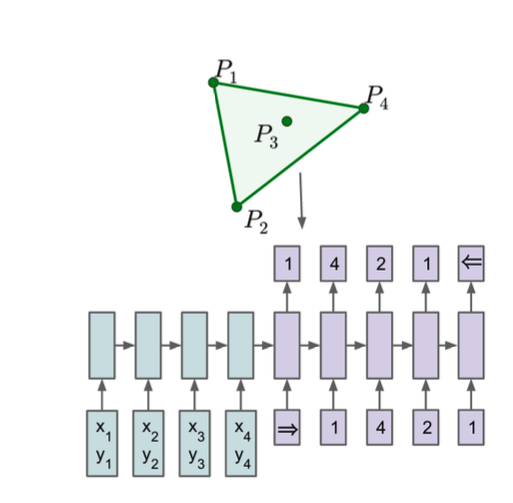
\includegraphics[width=0.5\textwidth]{Figures/seq.png}}\hfill
% \subfloat[Ptr-Net.\label{fig:1b}] {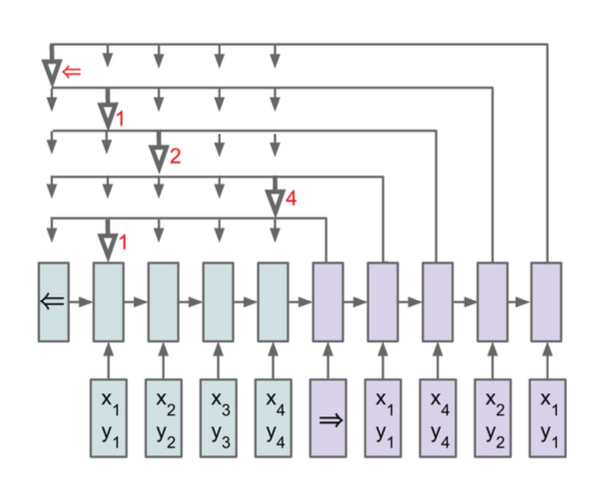
\includegraphics[width=0.5\textwidth]{Figures/soft_max.png}}
% \caption{Comparison of a Transformer (Sequence-to-Sequence model with a Ptr-Net.)~\cite{pointer}.} 
% \label{fig:pointer}
% \end{figure}

% By predicting words from the input sequence, Ptr-Nets offer a solution to the challenge of anticipating words that are not in one's vocabulary. However, Ptr-Nets can only anticipate words that appear in the local context because they cannot predict words outside of the input sequence (like a block of code).

% Due to this restriction, the Pointer Mixture Network, which predicts words either from the global vocabulary or copies one from local context, was introduced~\cite{ccnlm}. It combines Attention (long dependencies) and Ptr-Nets (local dependencies). In addition, a modified version of the Attention mechanism using an AST-based programming language was developed in this study~\cite{ccnlm}.

\subsection{GitHub Copilot}
In-IDE code completion tools have improved a lot in recent years, from suggesting variables or method calls from user code bases~\cite{mandelin2005} to suggesting entire code blocks~\cite{Ciniselli2021}. 
NLM-based approaches like Copilot have done remarkably well on improving the state-of-the-art in code completion, solving programming contest style problems~\cite{empirical_eval}.
GitHub's Copilot, which was released as technical preview in June 2021, is an in-IDE recommender system that makes use of OpenAI's Codex model, which employs a GPT-3 model, and is then optimized on code from GitHub to produce code suggestions~\cite{Copilot-web}. 
While many other research projects have attempted to do something similar~\cite{codesearch, natural, coacor}, Copilot's availability and smooth integration with GitHub's backup have unavoidably generated a ``hype" in the tech community, with many developers either already using it through its technical preview or started using it after its recent public launch as a paid subscription~\cite{Copilot-web}. 

Vaithilingam et al.~\cite{Vaithilingam2022} conducted an exploratory study of how developers use Copilot, finding that Copilot did not solve tasks more quickly, but did save time in searching for solutions. More importantly, Copilot seemed to solve the writer's block problem of not knowing how to get started. This notion of seeding an initial, if incorrect, solution is often how design proceeds in software. 

Currently, Copilot provides three key functionalities: autofill for repetitious code, tests suggested based on implementation code, and comment to code conversion~\cite{Copilot-web}. For the scope of this thesis, we focus on the first feature, which turns comments into code when a user adds a remark describing the logic they want to utilise~\cite{Copilot-web}. Although a Copilot suggestion can be triggered by by adding a comment in natural language, it is advised that users add descriptive comments and meaningful names for function parameters in order to receive useful recommendations~\cite{Copilot-web}. The Human Input is the concatenation of the natural language comment, function name, and function parameters.

Recent work shows initial investigations on how large language models for code can add architecture tactics by using program synthesis~\cite{Shokri2021} and structure learning~\cite{Karmakar2021}.
Our approach complements these earlier approaches by focusing on moving beyond code completion, where most research effort is currently concentrated.
In order to provide deeper insights into the overall effectiveness of the instrument, it is crucial to evaluate the quality of Copilot's suggestions and understand its limitations.

\subsection{Alternatives to Copilot}
There are a handful of code completion systems currently being used, below is a list a few such systems:

\begin{itemize}
    \item Jedi~\cite{jedi} - An open source python static analysis tool aimed at automatic code completion.
    \item Kite~\cite{kite} - Kite is an AI-powered code completion plugin that works with 16 languages and 16 IDEs.
    \item Deep TabNine~\cite{tabnine} - Deep TabNine is a source code completion system which is based on OpenAI's GPT-2 Model~\cite{gpt2}.
    \item AlphaCode~\cite{alphacode} - An \cct{} by DeepMind which uses a transformer language model to generate code, pre-trained on selected GitHub code and fine-tuning on a curated set of competitive programming problems~\cite{alphacode}.
    \item CodeBERT~\cite{codebert} - a bimodal pre-trained model for programming language (PL) and natural language (NL) by Microsoft. it uses multi-layer bidirectional Transformers for code completion~\cite{codebert}.
\end{itemize}
